\subsection[Prof. Dr. Christian Joppke] {Prof. Dr. Christian Joppke{\normalfont\normalsize\newline(Left IUB in July 2006)}}

\vspace{0.3cm}
\textbf{Main Research Interests}\\[-0.25cm]
\begin{enumerate}
\item[$\bullet$]	Immigration and Citizenship
\item[$\bullet$]	Ethnic Diversity Laws and Policies in Europe
\item[$\bullet$]	Institutional Accommodation of Islam in Europe and North America
\end{enumerate}


\vspace{0.6cm}
\textbf{Research Activities}\\[-0.25cm]

Between 1 January and 31 July 2006, Christian Joppke finished a research proposal, "Transformation of Citizenship in the Postnational State", for Collaborative Research Center "Transformations of the State" (directed by S. Leibfried and P. Genschel). It was favorably reviewed and suggested for inclusion in the CRC's request for follow-up funding from January 2008. In addition, Joppke finalized two articles, which he submitted for publication (outcome as yet pending). Christian Joppke also participated in the preparation of the proposal for a Bremen International Graduate School for Social Sciences in the framework of the Excellence Initiative; in it he functioned as a theme coordinator.
\begin{figure}[ht]
  \begin{center}
    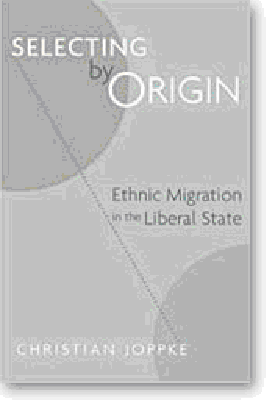
\includegraphics[width=5cm]{./SocSci/Joppke-fig001.pdf}
%   \mycaption{ xxx )}\label{fig:profxxx}
   \end{center}
\end{figure}


\vspace{0.6cm}
\textbf{PhD-Students}\\[-0.25cm]

Sara Geerdes\newline
\textit{Migration and Labor Market Transitions in selected European countries}
